%=========================================================================================================

\begin{quote}
	\textit{``If the chaos of the nineties reflects a radical shift in the paradigms of visual literacy, the final shift away from the Lascaux/Gutenberg tradition of a pre-holographic society, what should we expect from this newer technology, with his promise of discrete encoding and subsequent reconstruction of the full range of sensory perception?''}
\end{quote}
\hfill \textit{Burning Chrome, William Gibson}
\\
\\

%=========================================================================================================

\label{chapter-conclusions}

Alternate realities have fascinated mankind since early prehistory and with the advent of the computer and the smartphone we have seen the rise of many different categories of alternate reality that seek to replace, augment, diminish and mix with our familiar real world to expand our capabilities and our understanding. This thesis has introduced parallel reality as a new category of alternate reality comprising two environments that the user may freely switch between, one real and the other virtual, both complete unto themselves. The benefits that such a system impart upon the user by granting them the ability to mitigate the effects of an extended definition of the vacancy problem, first observed by Joshua Lifton during his investigation into the cross reality paradigm, and to explore parallel real and virtual environments in tandem have been shown through the development of the Mirrorshades parallel reality platform and its application to user studies within the realm of cultural heritage. Evaluation of these studies has lead to the establishment of a number of best practice recommendations to guide future parallel reality endeavours.

\begin{figure}[t]
	\begin{center}
		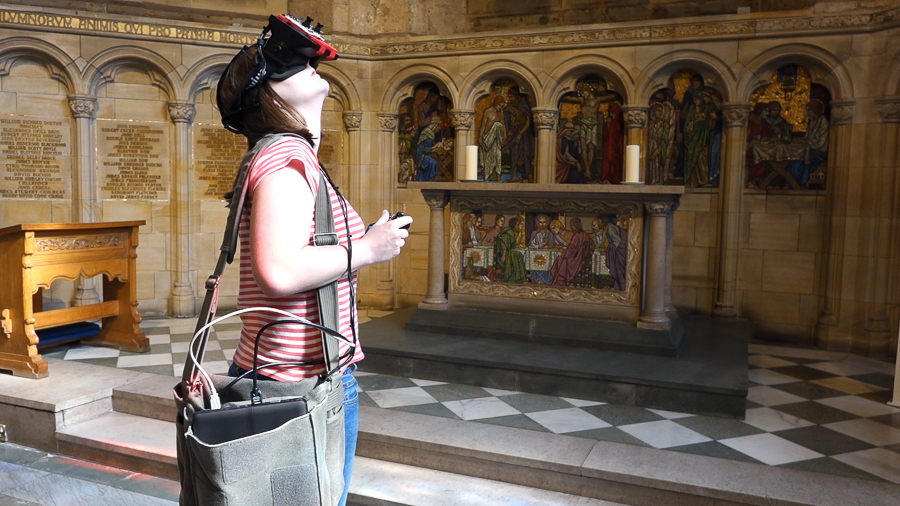
\includegraphics[width=\textwidth]{participant-f-4.jpg}
		\caption{The Mirrorshades parallel reality platform in use at a 15th century chapel.}
		\label{participant-f-4.jpg}
	\end{center}	
\end{figure}

\begin{figure}[t]
	\begin{center}
		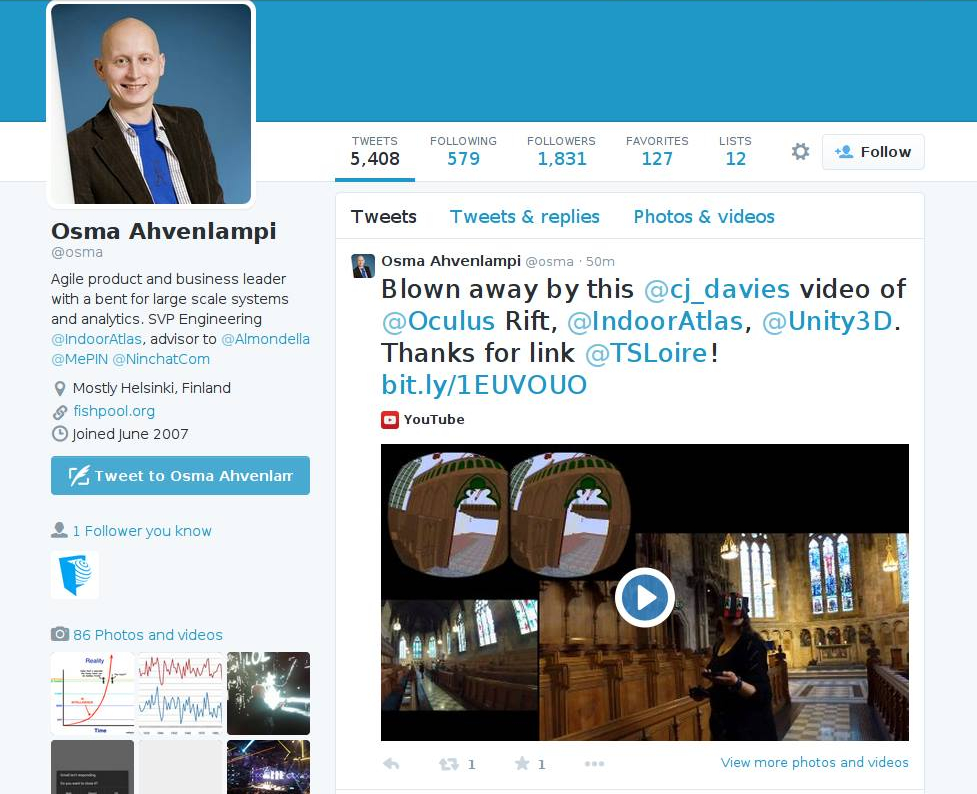
\includegraphics[width=0.8\textwidth]{osma-twitter.jpg}
		\caption{Praise for the Mirrorshades parallel reality platform from IndoorAtlas' senior vice president of engineering.}
		\label{osma-twitter.jpg}
	\end{center}	
\end{figure}

%=========================================================================================================

\section{Contributions}

As listed in section \ref{intro-contributions} the contributions of this thesis can be summarized at a high level as follows:

\begin{itemize}
	\item The introduction of parallel reality as a new category of alternate reality that allows users to experience complete real and virtual environments in tandem and represents an avenue for further mitigation of the vacancy problem.
	\item The framing of parallel reality through a thorough investigation and extension of previous taxonomies that classify and distinguish between alternate reality terminologies.
	\item The introduction of the combined Milgram/Waterworth model and the extended vacancy problem definition, for visualising alternate reality experiences, including those of parallel reality systems.
	\item Exploration into the suitability of an existing state of the art alternate reality modality of interaction (Situated Simulations) for investigation into parallel reality experience, producing the Virtual Time Window platform through extension of the Second Life client.
	\item Development of a bespoke platform for parallel reality, dubbed Mirrorshades, that uses the Unity game engine to combine the modern virtual reality hardware of the Oculus Rift with the novel indoor positioning technology of IndoorAtlas.
	\item Evaluation of the Mirrorshades platform through user studies of a real world use case studies within the realm of virtual heritage, including the discussion and application of an established presence questionnaire to a parallel reality experience, both to assess the worth of the concept and to inform future implementations.
	\item Creation and discussion of a set of best practice recommendations to guide future parallel reality endeavours.
\end{itemize}

%=========================================================================================================

\section{Objectives}

In reference to the objectives as originally listed in section \ref{objectivesandmethodology} this thesis has been successful in meeting what it set out to do, as discussed below.

\begin{enumerate}
	\item[1] Introduce the parallel reality concept by situating it within the larger ecosystem of existing categories of alternate reality, through a thorough exploration of existing alternate reality definitions, taxonomies and frameworks.
\end{enumerate}

The introduction of parallel reality as a new category of alternate reality in a clear and unambiguous fashion was no simple task, as decades of research into alternate realities has furnished us with a rich continuum of approaches and technologies for creating, combining, augmenting and diminishing real and virtual environments. The fact that there are often no clear boundaries between where one category ends and another begins, with the inherently subjective nature of space experience leading to continuums being a more popular method for identification than discrete categorisation, has lead to many common labels being applied to multiple subtly different scenarios. Whilst some of these uses are explained easily enough by differing subjective positions, some would seem at first glance to be almost contradictory.

The purpose of the extensive background and literature review in chapter \ref{chapter-background} into existing techniques for categorising and distinguishing between different alternate realities was thus to ensure that parallel reality could be introduced in a fashion that made its position clear and unambiguous when compared to all previous alternate reality terms. Naturally this review itself is contingent upon the author's own subjective positions and opinions, with such discussions of space experience at risk of leaning toward philosophy as much as they do toward computing, however the import of the endeavour was not to create a canonical set of definitions but rather to remove ambiguity in the introduction and definition of parallel reality.

\begin{enumerate}
	\item[2] Develop a suitable model for the illustration of experience in parallel reality scenarios, allowing not only for comparison and contrast between parallel reality and other alternate reality experiences, but also for illustration of different implementations of parallel reality experience.
\end{enumerate}

As one of the direct products of the work discussed for objective 1, the combined Milgram/Waterworth model (section \ref{combined-milgram-waterworth-model}) was produced for this purpose and represents a novel tool for visualising, discussing and comparing alternate reality experiences. By combining the relatively objective assessment of where the percepts a user is perceiving originate from (Milgram and Kishino) with the more subjective and experiential assessment of the direction and magnitude of that user's mental resources (Waterworth and Waterworth) we are gifted the ability to assess both vantages upon a single plot, which promises to make relationships between them more visible and more easily discussed.

One such relationship that became apparent in this manner was that of how the vacancy problem, as identified by Lifton in his cross reality research, can be mapped and explained in reference to both the Milgram and Kishino continuum and the Waterworth and Waterworth model, while also connecting with the Waterworth and Waterworth notion of the break in presence concept. This observation led to the introduction and definition of the extended vacancy problem, as found in section \ref{visualising-transitions-extended-vacancy} and reproduced below:

\begin{quote}
	\textbf{The Extended Vacancy Problem} - Performing a transition between two environments upon the locus of attention axis of the combined Milgram/Waterworth model is accompanied by a break in presence that manifests as a deflection upon the focus of attention axis from presence towards absence.
\end{quote}

The combined Milgram/Waterworth model is a particularly useful visualisation method for discussing the parallel reality concept, as the manner in which it allows the comparatively objective assessment of the provenance of the stimuli that the user is perceiving to be visualised along with the comparatively subjective assessment of their experience in terms of conceptual versus perceptual processing and their level of conscious arousal is of particular value for systems in which there is more than one environment that the user is encouraged to attend to, unlike the majority of previous alternate reality experiences wherein the user is encouraged to attend to a single environment (whether that be real, virtual, or a mix) at the intentional exclusion of all others.

\begin{enumerate}
	\item[3] Develop a parallel reality system suitable for deployment to real world user studies to effect comparison against previous categories of alternate reality.
\end{enumerate}

Initially it was thought that a rewarding parallel reality experience might be possible through leveraging an existing modality of alternate reality interaction, that of Situated Simulation (SitSim), and the VTW project discussed in chapter \ref{chapter-vtw} investigated this possibility. Evaluation of the VTW platform uncovered two major shortcomings.

The first was related to performance and was tied to the specification of the hardware and software platforms themselves, rather than being a result of any limitation imposed by the parallel reality concept itself. The decision to adopt the Second Life/OpenSim software environment, in order to make use of existing virtual content without having to embark upon a lengthy conversion process, limited the choice of tablet computer upon which the platform could operate to the very small number (at the time) of x86 tablet computers. None of these had the graphical performance of today's popular Android and iOS tablets which, when combined with the fact that Second Life/OpenSim is not in any way optimised nor designed for mobile use and is slower even than other non mobile 3D engines due to the ephemeral nature of its content, meant that graphical performance and quality were low.

The low performance and poor accessibility of the tablet's GPS and orientation sensing hardware also meant that a lengthy process of hardware prototyping and integration was required, and due to the limited control interfaces provided by the Second Life client it was necessary to embark upon a substantial software development stage, which resorted to adding low level serial I/O to the client. The observed performance of the position tracking obtained via the GPS receiver was then only sufficient to partially meet the requirements of the first and part of the second of the three envisaged styles of interaction with parallel reality systems as discussed in section \ref{parallel-reality-in-virtual-heritage}.

The second shortcoming of VTW was that the modality of interaction offered by the platform did not encapsulate that which was originally envisaged of the parallel reality concept of wholly switching between discrete real and virtual environments, due to the way in which the virtual was always seen as a small window surrounded by the larger and more encompassing real. When SitSim was being considered as a possible avenue through which parallel reality could manifest, the focus had been placed upon the environmental aspect, as the SitSim concept presented two complete and discrete environments, one real and the other virtual. It was not until testing the VTW platform at St Andrews Cathedral that the importance of the experiential aspect of the parallel reality concept also become clear. This led to the explicit realisation and appreciation of these two aspects of the parallel reality concept in section \ref{real-world-experience-of-vtw}, both of which needed to be realised in order for parallel reality to manifest in its originally envisaged manner.

The recognition of these shortcomings highlighted the importance of the experiential aspect of parallel reality, as well as providing insight into performance requirements and best practices over what software/hardware environment to make use of, and this information was used to influence the design and development of the subsequent Mirrorshades parallel reality platform.

While the physical manifestation of the Mirrorshades platform is less convenient and falls more into the category of `research equipment' than VTW, due to the fact that it fills a satchel that must be worn by the user and also occupies both of their hands with equipment, it fully realised the envisaged experience of parallel reality and did so with higher graphical performance and quality, along with higher orientation and position tracking quality thanks to the adoption of a more suitable software environment coupled with the (then) new Rift DK1 stereoscopic 3D HMD from Oculus. Using this platform it was then possible to perform user studies to assess the feasibility and worth of the concept and begin to ascertain properties and qualities of parallel reality experiences that effect their utility and enjoyment to guide future endeavours.

\begin{enumerate}	
	\item[4] Identify and put into practice suitable assessment techniques to ascertain the merit of parallel reality in relation to previous categories of alternate reality.
	\item[5] Identify aspects of the implementation of a parallel reality system that positively or negatively effect the user experience, along with assessment methodologies to ascertain these effects, putting these into practice within real world user studies.
\end{enumerate}

The inherently subjective nature of real and virtual space experience made such assessment techniques a challenge to decide upon. However with the utility of the combined Milgram/Waterworth model and the extended vacancy problem definition, a combination of both qualitative and quantitative techniques were identified that in combination would provide sufficient data to allow interesting observations and discoveries to be made (sections \ref{stage-1-evaluation-techniques} and \ref{stage-2-1-evaluation-techniques}).

The notion of presence in relation to parallel reality experiences presented an interesting challenge for assessment (section \ref{presence-questionnaires}), as the novel nature of a parallel reality experience in promoting interaction with two discrete environments rendered most popular presence questionnaires unsuitable. These questionnaires were written for assessment of traditionally realised virtual reality experiences, in which the user is immersed in a virtual environment at the intentional exclusion of all stimuli from the real world. However by realising that the design of the igroup presence questionnaire and its 3 categories allowed the novel aspect of a parallel reality experience when compared to a traditional VR experience to be isolated and assessed accordingly (section \ref{igroup-presence-questionnaire-explanation}), it could be applied to the new category of alternate reality and served to reinforce in a more scientific fashion what was being observed in some of the qualitative feedback.

\begin{enumerate}
	\item[6] Evaluate user studies to inform creation of best practise recommendations for future parallel reality endeavours.
\end{enumerate}

As listed in section \ref{best-practices-for-parallel-reality} a number of best practice recommendations to guide future parallel reality endeavours were created. These best practice recommendations are presented as observations from an initial investigation into a new category of alternate reality. The small number of participants, their limited age range and the use of a single case study within the context of cultural heritage prevents any detailed, low level claims being made into the best manners in which to implement particular features of a parallel reality system. But as initial evidence that justifies more detailed future work, they hope to help direct the design and implementation of future parallel reality endeavours without presumptuously attempting to prescribe specifics of individual features for which sufficient data and observations are not yet available.

These best practice recommendations cover technology based aspects, such as the importance of choosing appropriate hardware and software environments to provide the best graphical quality as possible, aspects mitigating limitations of technology that are not as easily overcome, such as intelligently handling inaccuracies in position tracking, as well as more subjective/experiential aspects relating to how implementation of transitions between real and virtual environments affect user experience, utility of the system and overall enjoyment.

%=========================================================================================================

\section{Emergent Preference Toward Mixed View}

The style of interaction originally envisaged for a parallel reality system was one of wholly switching between complete, discrete real and virtual environments, a scenario visualised upon the combined Milgram/Waterworth model in figure \ref{focus-locus-sensus-with-virtuality-continuum-with-transition}. After the experience of using the VTW platform fell short of this vision it was recognised in section \ref{real-world-experience-of-vtw} that the parallel reality definition could be considered as relying upon two aspects, the first focussing upon the provision of two complete environments, one real and the other virtual, and the second focussing on this experiential aspect of switching between these environments.

It was considered from the beginning that a scenario in which the user switches from a mixed real and virtual environment to a wholly virtual environment, as visualised in figure \ref{transition-mix-vr.png}, would be beneficial in terms of mitigating the effect of the extended vacancy problem. However it was not expected at that stage that users would come to prefer this mixed view to the extent that they did in the user studies when compared to the wholly real and wholly virtual views.

While the Mirrorshades platform succeeded where the VTW platform did not by allowing the envisaged style of interaction to manifest, the stage 2.1 evaluation indicated that users found the ability to view a mix of both real and virtual environments to be arguably more enjoyable and useful than the envisaged switching behaviour. The stage 2.2 evaluation was then designed partly to further investigate this observation and its results supported the finding.

At the very beginning of this thesis, in the introduction to chapter \ref{introduction}, the example scenario being described makes the following distinction about parallel reality:

\begin{quote}
	\textit{``This is not an augmented reality system which superimposes virtual objects upon the real world.''}
\end{quote}

And later when formally introducing parallel reality in section \ref{parallelrealityinbackground} this thesis explained:

\begin{quote}
	\textit{``In this regard we further distinguish a parallel reality system from an augmented reality system by defining the former as allowing its user to switch between two different primary environments whereas the latter augments one particular primary environment.''}
\end{quote}

With the emergent preference of users in the Mirrorshades parallel reality platform evaluations towards a mixed view, the novelty of parallel reality as a distinct category of alternate reality is definitely put into question, as the user experience of the Mirrorshades platform as used in this fashion is undeniably very similar to previous AR platforms.

However, in reference to section \ref{real-world-experience-of-vtw}, even though the experiential aspect of the parallel reality platform in this mixed view scenario is difficult to distinguish from an AR platform, the distinct environmental aspect of the parallel reality platform means that it should still be considered a distinct concept due to the utility it provides to additionally alter the experiential aspect away from a mixed view where this becomes desirable.

The provision of a complete virtual environment means that the user of a parallel reality system who is viewing a mixed real/virtual view can at any time transition to seeing only real or only virtual, something that is not encapsulated by the popular definition and understanding of AR (see section \ref{summaryofalternaterealitydefinitions}) as being a single mixed environment created by the addition of some virtual objects to the real environment, wherein the virtual objects alone do not constitute an entire environment and rely upon their juxtaposition upon the real environment.

As mentioned in section \ref{stage-2-2-summary}, this observed preference toward a mixed view indicates that the ultimate realisation of the parallel reality concept may be one that provides the ability to view such a mix, possibly even as the default view, but which \textit{additionally} allows the user to transition into viewing purely real and purely virtual environments on their own at the complete exclusion of the other, in order to perform more detailed observation of particular aspects and to aid in ambulation. One might want to consider this realisation of parallel reality as being an extreme case of AR, in which the quantity and coverage of the virtual objects surpasses that expected from the traditional understanding of AR and trends toward a point at which they do in fact constitute a complete virtual environment and thus become part of a parallel reality system.

The predisposition toward continuums, rather than categories with discrete boundaries, when discussing the position of different categories of alternate reality in relationship to each other, lends well to this possibility, producing the idea of a categorisation system where an AR system with an increasing coverage of virtual objects trends along a continuum toward a point at which it can be considered to be a parallel reality system, as shown by figure \ref{augmented-reality-parallel-reality-continuum.png}.

\begin{figure}[h]
	\begin{center}
		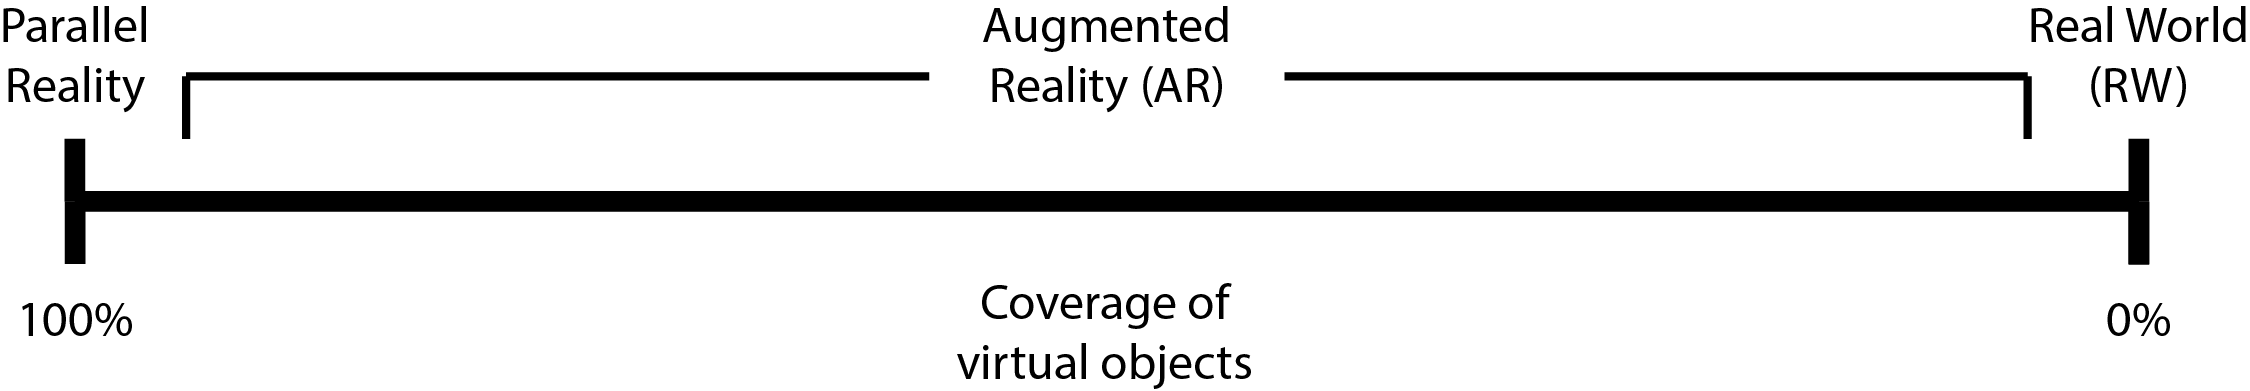
\includegraphics[width=\textwidth]{augmented-reality-parallel-reality-continuum.png}
		\caption{Continuum of increasing coverage of virtual objects in AR trending toward parallel reality classification.}
		\label{augmented-reality-parallel-reality-continuum.png}
	\end{center}	
\end{figure}

%talk about how the real made the virtual look more realistic, as being possible in parallel reality but not in AR

%=========================================================================================================

\section{Future Work}

The introduction of parallel reality in this thesis along with the evaluation of its first involved implementations, which investigated leveraging an existing modality of alternate reality interaction with VTW and explored a novel new style of alternate reality interaction with Mirrorshades, is only the beginning of an extended course of study that will be required to fully understand and come to appreciate the benefits that it can provide as a concept. The following discussion highlights but a few choice avenues that the future investigation of parallel reality would do well to explore and should by no means be considered an exhaustive list of possible sources of extension; after all the \textit{``potential applications of VR are really only limited by the imaginations of talented individuals''}~\cite{Giuseppe2014a}. Since its recent rejuvenation at the hands of Oculus, the field of virtual reality has seen its rate of progress and advancement massively accelerated. With this in mind, the potential of these avenues for further investigation into the parallel reality concept to produce fruitful results is substantial.

Most evident is the matter of hardware. The Mirrorshades parallel reality platform used in the user studies presented in this thesis is a somewhat cumbersome package of HMD, laptop, battery pack, smartphone, games console controller and myriad cables, occupying both of the user's hands and requiring them to carry a satchel of not insubstantial size and weight (large enough for an 11`` laptop and around 2.5kg in total). To posit that the cumbersome nature of the platform had a directly detrimental effect upon the quality of experience received by the participants is no stretch of the imagination and improvements in this regard will be required for parallel reality to see deployment and use in anything but controlled laboratory or user study conditions. As discussed in section \ref{mobile-client} we are already beginning to see the advent of hardware platforms that present a much improved basis for parallel reality experiences. A platform such as Samsung Gear VR, perhaps modified with stereoscopic video see-through abilities, would represent a fully contained single unit parallel reality experience, suitable for handing to a user in the same manner that audio guides are given out at many of the world's museums. Google's Cardboard platform\footnote{\url{https://www.google.com/get/cardboard/}} also presents an intriguing possibility for future parallel reality implementations at very low cost, making use of nothing more than a folded piece of cardboard and two plastic lenses combined with any of a wide variety of smartphones to form a rudimentary HMD which users could bring to their eyes to perform a transition into VR and remove when they wish to view their real surroundings. Furthermore, improvements to the performance of the platforms, in terms of the visual acuity of both real and virtual content as well as the accuracy of the positioning and registration, will present beneficial results both to casual users and to experts wishing to use such a modality of interaction for serious study. 

Investigating the application of parallel reality to other domains represents possibly the largest avenue of potential extension. While the user studies discussed in this thesis experimentally demonstrated the worth of parallel reality when applied to the field of cultural heritage, parallel reality as a concept can be applied to many fields. Postulating for but a moment one can imagine how parallel reality could be applied to architecture to allow people to walk through a house as it is still being built or renovated and switch to seeing its destined form, to using the physical layout of an environment as a canvas for novel artistic expression, to the study of polysocial interactions involving real and VR parties, to new styles of gaming that merge both real and virtual play fields, to allowing rescue workers to study the state of a building before a fire broke out and identify dangers that could now be hidden in the flames. As society becomes both more familiar with and more dependent upon almost constant connection to the virtual, whether in the form of 2D Web based social networks and apps or richer multimedia experiences, the utility of platforms that allow real and virtual environments to be cycled between in a trivial manner will present many exciting applications for parallel reality, including in as yet unforeseen areas. Parallel reality could even help move us closer to a future akin to that described by Vernor Vinge in \textit{Rainbows End}, in which layers of 3D virtual content are always available to be browsed and to transform and exploit the real world environment, whether it happens to be the playground or the office.

In addition to other domains the application of parallel reality systems to more expansive environments should also prove to be a fruitful avenue of investigation. In the Mirrorshades evaluations participants were restricted to the area within St Salvator's chapel, however from a conceptual perspective there is nothing to prevent parallel reality from being deployed on larger scales. Allowing the user of a parallel reality system to move between indoor and outdoor areas would require the integration of multiple positioning systems, at least one for indoor areas and a second for outdoor areas. As the virtual environment grows in tandem with the increasing area of the real world available for the user to roam within a switch from static content stored upon the local client to content dynamically streamed from the cloud would likely be required.

Furthermore when considering evaluation, the experience of using a parallel reality system has been assessed in this thesis only in relation to a seated VR experience within a cultural heritage scenario and with a focus upon the presence perspective. This represents only a small foray into the sources of study and evaluation that could (and perhaps should) be applied to parallel reality systems, especially when one considers applications in different domains, on larger scales and with the introduction of other users, both real and virtual, local and remote.

Finally, the evaluation of parallel reality in this thesis has been based upon experiences with a parallel reality system that features high spatial equivalence (see section \ref{spatial-equivalence}) between its real and virtual environments. The application of parallel reality to scenarios that feature little or no spatial equivalence between their environments will surely open up a wealth of exciting investigations requiring markedly different approaches to both implementation and evaluation. This situation may become particularly pertinent as the promise of VR for social activities grows, possibly bringing us to a near future situation similar to that exemplified by the quote from Neal Stephenson's \textit{Snow Crash} at the beginning of chapter \ref{chapter-background}; a future world where a multi user 3D virtual environment accessed via HMD, but which has no partner in the real world, commands so much of our attention that people find themselves wanting to constantly be able to switch between one and the other to maintain a presence in each.

In summary, future research into the parallel reality concept would do well to:
\begin{itemize}
	\item Investigate its application to other domains, in particular those in which previously established alternate reality techniques have demonstrated success or in which previously established alternate reality techniques were not able to fulfil the hopes and expectations.

	\item Investigate its application over substantially larger environments, requiring adoption of smaller, lighter hardware and position tracking accurate over wide areas.

	\item Evaluate it from perspectives other than presence, perhaps focussing on utility when applied to particular tasks or challenges.

	\item Explore further the value and merit of switching wholly between real and virtual environments, taking into consideration the emergent preference of users toward an AR reminiscent mixed view, identifying where the new ability of parallel reality may improve scenarios that had previously made use of AR.
\end{itemize}
%=========================================================================================================

\section{Final Thoughts}

While mankind may still be many decades away from the realisation of a Neil Stephenson-esque metaverse, in which a persistent 3D multi-user virtual environment forms the basis for all of our computer mediated communication and commands as much of our attention as our smartphones do today, the parallel reality concept introduced by this thesis has provided a glimpse of how a novel new category of alternate reality can already allow us to interact in tandem with both an immersive 3D environment and the real world around us. While such a platform can already claim some small success in improving the experience of virtual heritage content, the possible applications of such a technology will surely only expand as we continue to integrate more virtuality into our daily lives and come to question our experiences as Orlan once proposed (emphasis original):

\begin{quote}
	\textit{``I come back therefore to my initial words about the `\textbf{and}' in order to propose the virtual \textbf{and} the real used simultaneously as new transversalities that question art and the becoming of our world.''}~\cite{Orlan2002}
\end{quote}

%=========================================================================================================